\section{Vocabulary with n-grams of up to length 4} \label{appendix_ngram_vocab}

Entries of the vocabulary are extracted from the text as n-grams, which are sequences of tokens of length $n$. To decide on the maximum length of the n-grams we want to extract, we have a look at an existing scientific vocabulary, EuroSciVoc\footnote{\url{https://op.europa.eu/en/web/eu-vocabularies/euroscivoc}}. It contains around a 1,000 scientific fields in several European languages. Including synonyms and related fields of studies, there are 3,494 entries in the vocabulary. 38 \% of them consist of one word and 50 \% of them comprise two words. Only 8 entries are longer than four words.

Given the importance of disposing of a thorough vocabulary, we will keep all n-grams up to those of length four. The ones that only occur once in the corpus will be removed at the end, as they cannot be used to relate documents. We also discard n-grams that contain a punctuation sign that signifies a break in the sentence (i.e. one of these: ``.'', ``,'', ``?'', ``!''). Such n-grams don't form valid phrases.

All n-grams of lengths 2 to 4 amount to many entries in the vocabulary. To reduce its size, we implemented a thorough filtering procedure that removes all entries that are redundant. This procedure is detailed in the following section. Afterwards, we present the resulting vocabulary, before and after filtering. Then, we briefly talk about the execution time of the filtering procedure.


\subsection{Vocabulary filtering} \label{vocab_filtering_ngrams}

Once the vocabulary has been created, we remove the entries that occur in only one document, as they cannot be used to relate documents. We also remove the entries that occur in more than 1,000 documents. We assume that their meanings are too broad and that they are thus not relevant for the task of subject indexing. Entries that are either stop words\footnote{For this purpose, we use NLTK's list of English stop words, which comprises 179 words as of 07/07/2021.} or punctuation signs are also discarded. This is the first step out of four that comprise our filtering procedure.

We remove entries that appear as many times (step 2) or one time more (step 3) than entries that contain them, as they only provide meaning when used with other words. For example, if ``supervised'' and ``supervised learning'' both occur 100 times, ``supervised'' should be removed. Also, if ``supervised'' occurs 101 times it should also be removed, as it only occurs once without being in ``supervised learning'' and thus belongs to the set of entries that cannot be used to relate documents.

Lastly, on step 4, we remove entries that either never occur alone or only once. For each entry, we find all the entries that include it. If the sum of their frequencies equals the frequency of the entry or is off by one (i.e. one less), we remove the entry. For example, if ``learning'' appears 100 times, ``supervised learning'' appears 40 times and ``machine learning'' appears 60 times, ``learning'' never occurs alone and should be removed. This step is computationally much more costly than the previous one, as all the remaining entries must be checked. This is why it is performed last.

It is important to note that the matches between entries are performed on the basis of tokens, not raw strings. The latter could lead to spurious behavior such as removing ``selling'' because it occurs as many times as ``counselling'', although they are different words.

\subsection{Resulting vocabulary}

In this section, we will present some facts about the vocabulary that arises from the procedure described above. We first look at the vocabulary before applying the filtering procedure described in section \ref{vocab_filtering_ngrams}, then look at its impact and the final vocabulary.

\subsubsection{Before filtering}

Before filtering, there are 8,892,623 entries in the vocabulary. As shown in figure \ref{fig:vocab_before_words}, almost half of them comprise four words (46 \%), while more than a third (36 \%) comprise three words. 15 \% of them consist of two words and 1.4 \% of them are singular words. This distribution makes sense, as there are fewer duplicates in larger n-grams than in singular words.

\begin{figure}
  \begin{subfigure}[t]{0.45\textwidth}
    \centering
    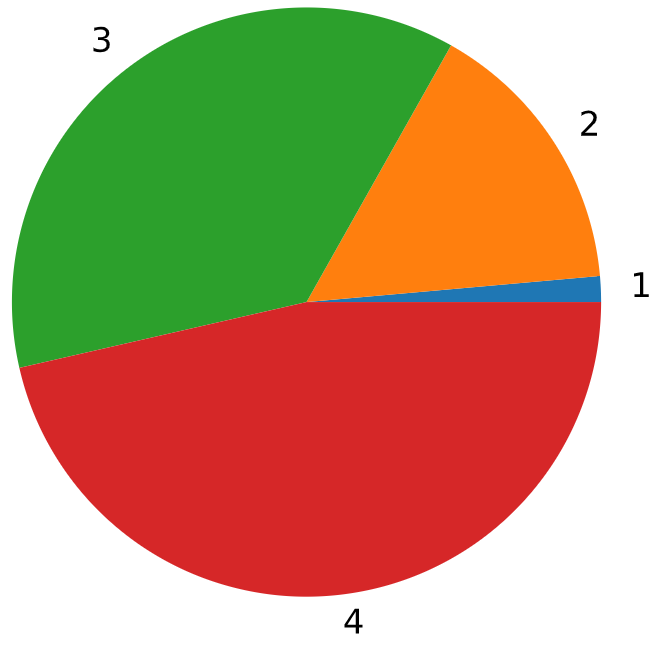
\includegraphics[width=\textwidth]{figures/vocab/before/n_words.PNG}
    \caption{No. of entries per no. of words.}
    \label{fig:vocab_before_words}
  \end{subfigure}
  \hfill
  \begin{subfigure}[t]{0.48\textwidth}
    \centering
    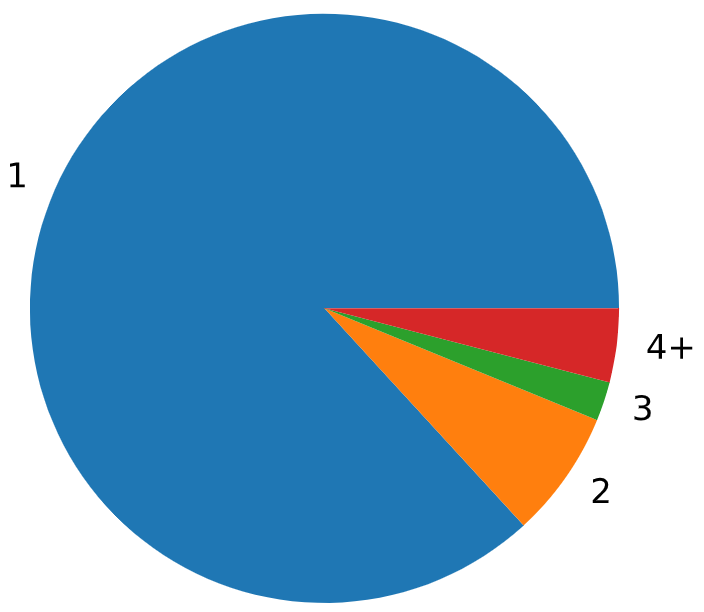
\includegraphics[width=\textwidth]{figures/vocab/before/entry_frequency.PNG}
    \caption{No. of entries per frequency (i.e. in how many documents they appear).}
    \label{fig:vocab_before_freq}
  \end{subfigure}
  \caption{Charts about the vocabulary before filtering.}
\end{figure}

87 \% of them appear only in one document, as illustrated in figure \ref{fig:vocab_before_freq}. 94 \% of the entries that comprise four words occur only once, while only 60 \% of the entries that are singular words are used in only one document. Entries with two and three words occur only once in 71 \% and 86 \% of the time. These percentages are inversely proportional to the number of entries per number of words that the entry has. This also makes sense, given that 4-grams rarely occur more than once (i.e. only when there is an actual scientific term that is this long or if there is a common sequence of four words, such as ``as well as the'', which occurs in 1,132 documents.).

There are 733 entries that occur in more than 1,000 documents. 487 of them (66 \%) comprise only one word. Only one of these entries consists of four words. The list includes words such as ``common'', ``research'' and ``thesis''. These words, although meaningful, occur too often in our dataset to be of any use for the task of semantically relating documents.

\subsubsection{After filtering}

The filtering procedure reduced the size of the vocabulary from 8,892,623 to 754,889 entries. The first step, in which the entries that occur either in one or in more than 1,000 documents are removed, had the largest effect, removing 7,720,983 entries. All but 733 of them are entries that occur only in one document, as was stated in the previous section.

Step 1 is also the only step in which 4-grams were removed, as shown in figure \ref{fig:words_per_entry_per_step}. As 4-grams are the largest n-grams in our dataset, they are not included in any other n-grams and thus cannot be removed by any of the following steps. No entries were removed during step 3, where entries that occurred once more than larger entries that contained them were filtered. This step is therefore not shown in the figures \ref{fig:words_per_entry_per_step} and \ref{fig:avg_frequency_per_step}. 

Figure \ref{fig:avg_frequency_per_step} shows the average frequency of the entries before the filtering procedure and after each step. The avg. frequency increased dramatically after step 1, where all the entries that only appear in one document (which comprise 87 \% of all entries) were removed. After step 4 the average frequency is 4.2, meaning that entries appear on average in around four documents.

Figures \ref{fig:vocab_after_words} and \ref{fig:vocab_after_freq} are equivalent to figures \ref{fig:vocab_before_words} and \ref{fig:vocab_before_freq} but for the filtered vocabulary. Figure \ref{fig:vocab_after_words} shows how the proportion of 4-grams has decreased, whereas the proportion of 2-grams has increased. Figure \ref{fig:vocab_after_freq} no longer includes entries that occur in only one document, as these were removed in step 1 of the filtering procedure. Almost 60 \% of the entries of the filtered vocabulary appear in two documents, while 18 \% appear in five or more documents.

\subsubsection{Execution time of the filtering procedure}

Regarding the performance of the filtering procedure, the first step is by far the fastest, taking only a couple of seconds. Steps 2 and 3 took around two days each, as the entries are grouped by frequency and each entry has to be compared with all the entries in their group. Step 3 took around eight hours less than step 2, as all the entries removed in step 2 were no longer considered. Step 4 took more than six days, as all entries are considered, not only the ones that belong to the same group.

\begin{figure}
  \begin{subfigure}[t]{0.5\textwidth}
    \centering
    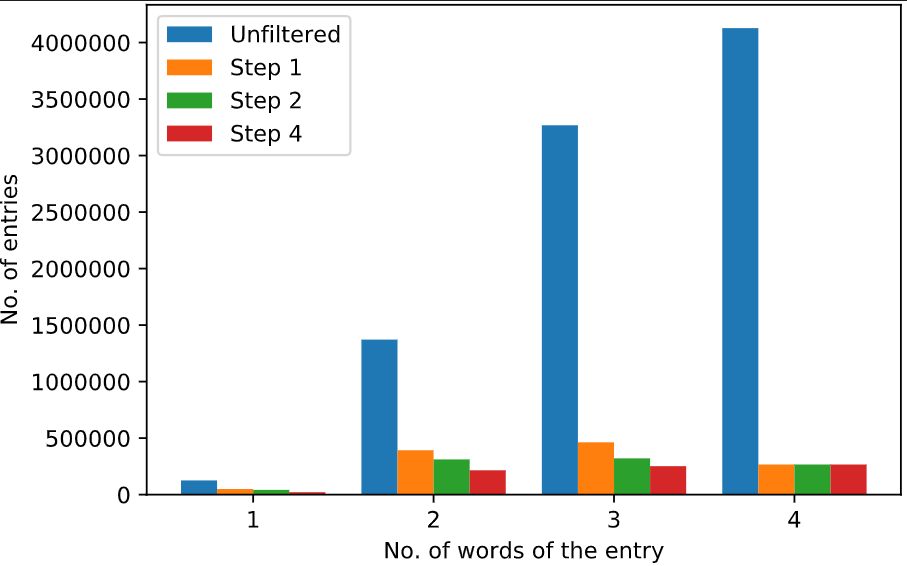
\includegraphics[width=\textwidth]{figures/vocab/after/words_per_entry_per_step.PNG}
    \caption{No. of entries per no. of words for each step.}
    \label{fig:words_per_entry_per_step}
  \end{subfigure}
  \hfill
  \begin{subfigure}[t]{0.48\textwidth}
    \centering
    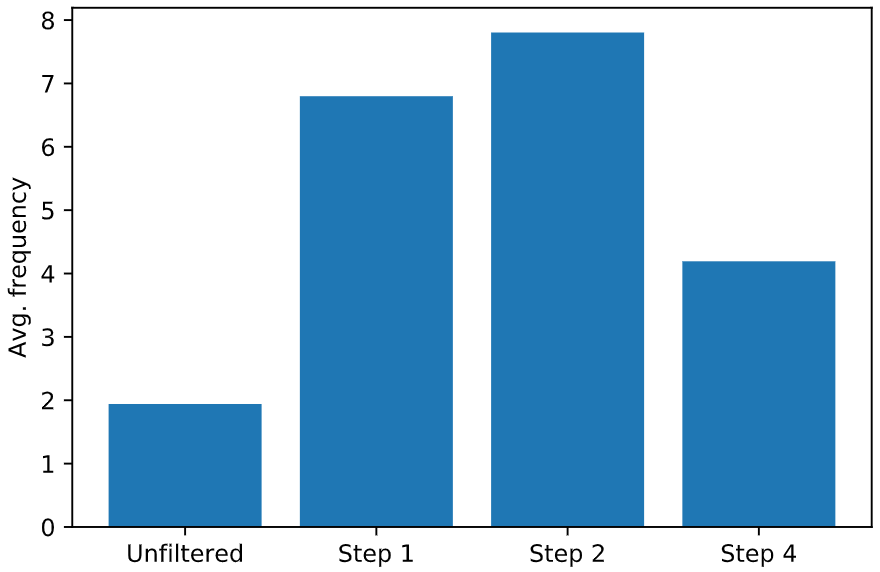
\includegraphics[width=\textwidth]{figures/vocab/after/avg_frequency_per_step.PNG}
    \caption{Avg. frequency of the entries after each step.}
    \label{fig:avg_frequency_per_step}
  \end{subfigure}
  \caption{Charts about the steps of the vocabulary filtering procedure.}
\end{figure}

\begin{figure}
  \begin{subfigure}[t]{0.52\textwidth}
    \centering
    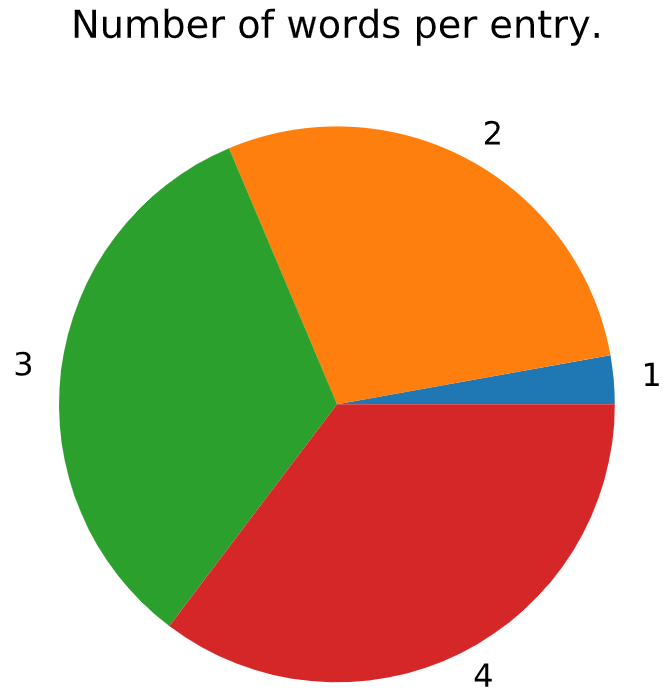
\includegraphics[width=\textwidth]{figures/vocab/after/words_per_entry.PNG}
    \caption{No. of entries per no. of words.}
    \label{fig:vocab_after_words}
  \end{subfigure}
  \hfill
  \begin{subfigure}[t]{0.44\textwidth}
    \centering
    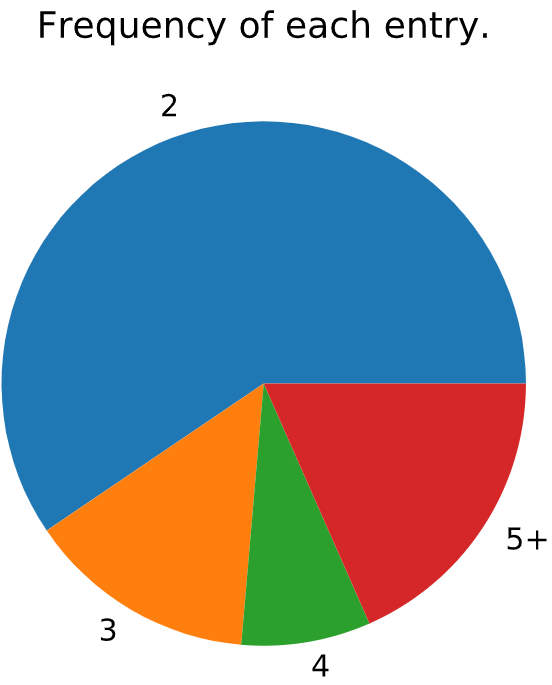
\includegraphics[width=\textwidth]{figures/vocab/after/entry_frequency.PNG}
    \caption{No. of entries per frequency (i.e. in how many documents they appear).}
    \label{fig:vocab_after_freq}
  \end{subfigure}
  \caption{Charts about the vocabulary after filtering.}
\end{figure}

\subsubsection{Quality of the vocabulary}

We have qualitatively assessed how useful the n-grams of the vocabulary are for our task. Unfortunately, most of the ones we have evaluated are uninformative. They are sequences of words that are often written together, but that don't have any special meaning. Examples of these are ``more general question'' and ``discuss the following''. We therefore discard them altogether, given that they dramatically increase the size of the vocabulary.